A plugin system was integrated into \sh to support calculation of properties for the molecules of a dataset.
\sh provides a basic set of built-in plugins, and the plugin system allows users to write calculation plugins suited to their particular needs.
%If you are familiar with programming in \software{Java}, you can write your own calculation plugins.
See \chapref{chap:scaffoldhunter:writeplugins} for a detailed description how to write a plugin.\\

\begin{figure}[!htb]
   \centering
   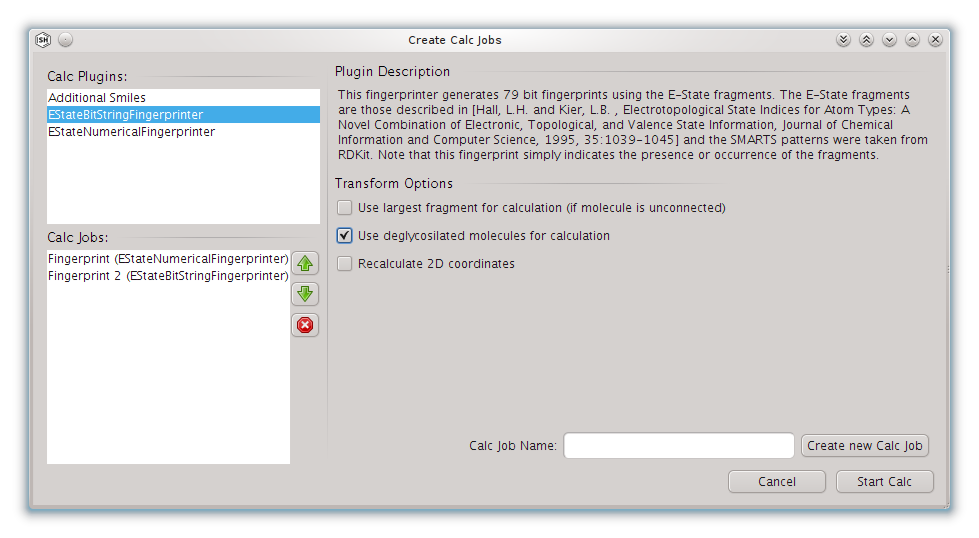
\includegraphics[width=\textwidth]{images/sh_create_calc_job_dialog.png}
   \caption{Create Calc Job Dialog}
   \label{fig:createcalcjobdialog}
\end{figure}

In the \guidialog{Create Calc Job Dialog} shown on \figref{fig:createcalcjobdialog} you can create a batch of calc jobs,
that should be executed one after each other.
Each calc job is an instance of a calc plugin, which is configured based on your needs.
Each plugin instance obtains a list of all molecules with their structural data and their existing properties,
and can use this data to calculate new properties for all (or some) molecules.
To create a batch of calc jobs, perform the following steps:

\paragraph{1. Select a calc plugin}
  In the top-left corner of the dialog you will find the list of calc plugins.
  Select one by clicking on it and proceed with the next step.

\paragraph{2. Configure the calc plugin}
  As you selected a calc plugin, the configuration panel on the right hand side of the dialog will show the plugin description
  and, depending on the plugin, a bunch of options to adjust the plugin.
  Choose the options you would like to use, and proceed with the next step.

\paragraph{3. Add the configured plugin to the list of calc jobs}
  After you have finished configuring the plugin, you can make the configured plugin instance a calc job.
  To do this, click on \gui{Create New Calc Job} in the bottom-right corner of the dialog.
  If you want to give the calc job a name, enter it in the text field labeled \gui{Calc Job Name} first. Otherwise leave the field blank.
  Now the calc job of the chosen name (or a default name) appears in the list of calc jobs in the bottom-left corner of the dialog.
  Proceed with step 1 if you want to add another calc job.

\paragraph{4. (optional) Edit the list of calc jobs}
  The list of calc jobs defines the order in which the jobs are executed.
  To change the order, select a calc job and move it up or down using the arrow buttons.
  To delete a calc job, select it and delete it by clicking on the \gui{X} button.
  If you want to change the configuration of a calc job, select it.
  The configuration panel on the right hand side of the dialog then lets you modify the job.\\

If you are ready to start the calculation, click \gui{Start Calc}.
If you want to return to the previous dialog without any changes on your dataset, click \gui{Cancel}.
After you have started the calculation, a progress window as shown in \figref{fig:calculationprogress}
will appear and inform you about the calculation status and possible issues during calculation.

\begin{figure}[!htb]
   \centering
   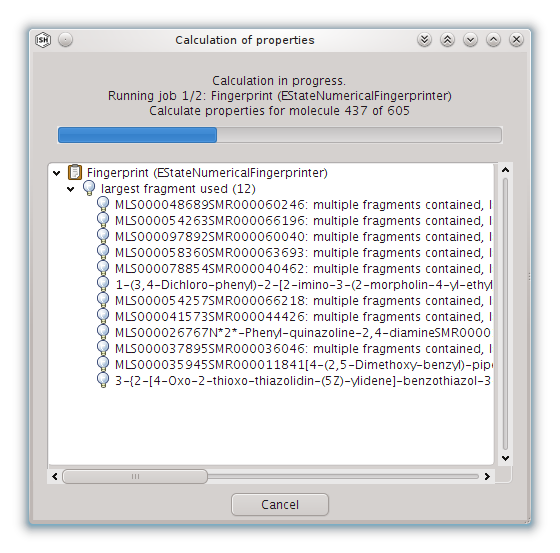
\includegraphics[scale=0.6]{images/sh_calculation_progress_dialog.png}
   \caption{Calculation Progress}
   \label{fig:calculationprogress}
\end{figure}

	
\subsubsection{Transform Options} \label{subsec:scaffoldhunter:Transform Options}
In addition to the specific options provided by each plugin, there are several plugins that provide transform options.
Transform options are used to transform the structure of all molecules, before the plugin starts the calculation.
The following transform options are available:
\paragraph{Use largest fragment}
  Sometimes multiple molecule fragments are stored (unconnected) in one single structure.
  If, for example, the plugin calculates a fingerprint which takes the molecular structure into account,
  you may want just the largest fragment of the compound to be used for the calculation.
		      
\paragraph{Use deglycosylated molecules}
  Perhaps deglycosylation (Read \subsecref{subsec:scaffoldhunter:deglycosylate} for an explanation of deglycosylation)
  has an effect on the accuracy of a calculated fingerprint.
  In this case you may want to deglycosylate before the calculation.

\paragraph{Recalculate 2D-coordinates}
  Some calc plugins (e.g. fingerprints) may depend on the 2D-coordinates of the molecules.
  If you are not sure whether all imported molecules have appropriate 2D-coordinates,
  you propably want to recalculate them for all molecules before calculating the fingerprint.


\subsubsection{Calc plugins}
Currently there are just three calc plugins available;
one plugin to calculate additional SMILES strings, and two plugins to calculate fingerprints which can be used for clustering of molecules.
Each plugin supplies its own description, so just select a plugin from the list of calc plugins as shown in \figref{fig:createcalcjobdialog} and consult the plugin description for an explanation of what the plugin does.
